\documentclass[../main.tex]{subfiles}

\begin{document}


\section{Practical performance}
\label{section:analysis:pratic_performance}
\par Now that we have seen how LAUXUS works, we will look at its performance to know the overhead occured. As a quick reminder, we don't want LAUXUS to cause a massive overhead compared to using the classical UNIX Filesystem. This is why, we will compare each LAUXUS operation with the corresponding operation on the UNIX Filesystem.
\par There will not be many measurements as we mainly want (in term of performance) LAUXUS to:
\begin{itemize}
    \item Cause a slight overhead to the write operation which may be high due to the encryption cost.
    \item Cause a slight overhead for the user entitlement when the file is deep inside the Filesystem hierarchy.
    \item Cause a slight overhead between editing a few bytes in a big or a small file.
\end{itemize}


\subsubsection{Copying operation overhead}
\label{section:analysis:write_overhead}
\begin{figure}[h]
    \centering
    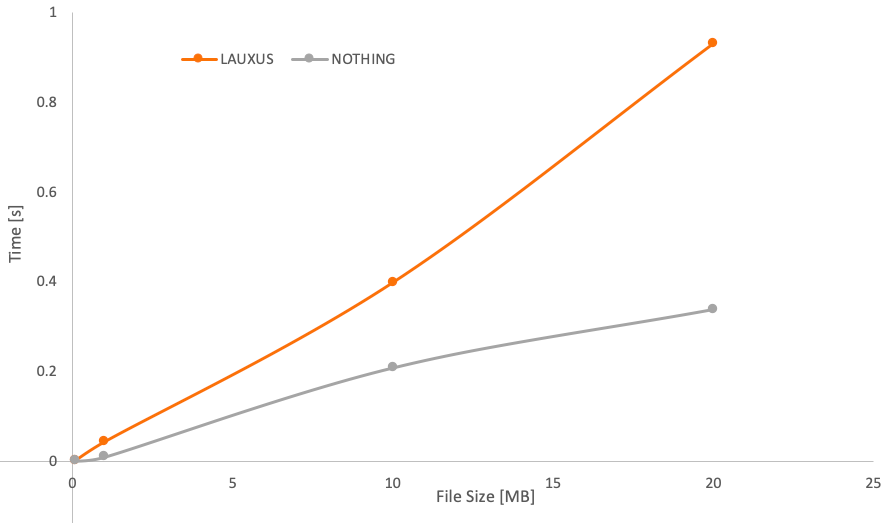
\includegraphics[width=.8\textwidth]{images/analysis/perf_write_per_size}
    
    \caption{Copying time VS Size of the file}
    \label{figure:analysis:perf_write_per_size}
\end{figure}
\par As we can see from the above Figure, we have a fairly slight overhead (only two times slower).  Furthermore, we see that the time taken evolves nearly linearly. This is very promising for very big file, which consequently should not take too long. From the design description, it is logic to have a linear evolution. Upon closer look, we see that the curve is not absolutely linear. This is because the size of the metadata structure increases throughout the copy operation. Further explanation on this behaviour is discussed in the Appendix \ref{appendix:additional_perf}.


\subsubsection{User entitlement overhead}
\label{section:analysis:user_entitlement_overhead}
\begin{figure}[h]
    \centering
    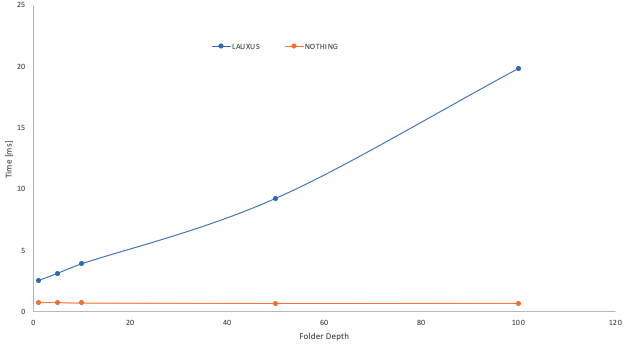
\includegraphics[width=.8\textwidth]{images/analysis/perf_write_per_depth}
    
    \caption{Copying time VS Depth of the file}
    \label{figure:analysis:perf_write_per_depth}
\end{figure}
\par This test is important because we have user entitlement on each directory. Furthermore, because the names of the files are obfuscated, we must load the parent directory of the concerned file. Indeed, each Dirnode contains a mapping between each of its children and their corresponding UUID. Furthermore, in order to find this last Dirnode UUID, we must find its parent directory and so on until we reach the root directory.
\par This means that theoretically, the deepest in the hierarchy the file is (number of parent directory to the root), the more we need to check the user entitlement and load node, increasing the overhead on the write operation. Which means, we except a linear evolution compared to the depth of the file. Fortunately, this process is done only done one time: when the file is opened. After opening, the file structure stays in memory and we no longer need to check all hierarchy nor too load the parent directories to find the Filenode's UUID.
\par The Figure \ref{figure:analysis:perf_write_per_depth} illustrate the above theoretical explanation.
\par We see that this cause a huge overhead when there is a lot of directories. Fortunately, inside a standard end-user Dropbox Filesystem, there are way fewer directories than 200. Overall, this overhead is very negligible and doesn't require any specific improvement.


\subsubsection{Writing few bytes overhead}
\label{section:analysis:write_offset_overhead}
\begin{figure}[h]
    \centering
    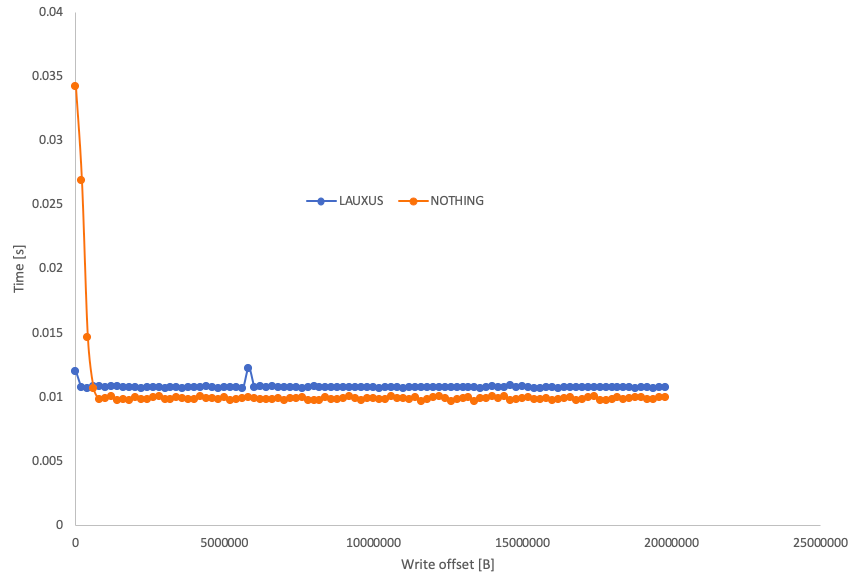
\includegraphics[width=.8\textwidth]{images/analysis/perf_write_per_offset}
    
    \caption{Writing few bytes at different offset inside a 20MB file}
    \label{figure:analysis:perf_write_per_offset}
\end{figure}
{???????????????????????????,,}



\end{document}